% Step 1 notes: queries, scores and filters.
% Build from this folder:  tectonic notes.tex
\documentclass[11pt]{article}
% Look and feel for the Step 1 notes. The main text is in notes.tex.
% Only the typeface block changes between design variants.

\usepackage{fontspec}
\usepackage[a4paper, left=2.7cm, textwidth=13.2cm, marginparsep=0.7cm,
  marginparwidth=4.0cm, top=3.0cm, bottom=3.2cm]{geometry}
\usepackage{xcolor}
\usepackage{booktabs}
\usepackage{tabularx}
\usepackage{amsmath}
\usepackage{amssymb}
\usepackage{enumitem}
\usepackage{listings}
\usepackage{tcolorbox}
\tcbuselibrary{skins}
\usepackage{marginnote}
\usepackage{tikz}
\usetikzlibrary{arrows.meta, positioning, calc, fit, shapes.geometric}
\usepackage{caption}
\usepackage{float}
\usepackage[hidelinks]{hyperref}

% ---- typeface (the design axis) -----------------------------------
\setmainfont{EBGaramond}[Extension=.otf, UprightFont=*-Regular, BoldFont=*-Bold, ItalicFont=*-Italic, BoldItalicFont=*-BoldItalic]
\newcommand{\fontlabel}{EB Garamond}

\setsansfont{texgyreheros}[Extension=.otf, UprightFont=*-regular,
  BoldFont=*-bold, ItalicFont=*-italic, BoldItalicFont=*-bolditalic,
  Scale=0.88]
\setmonofont{lmmono10}[Extension=.otf, UprightFont=*-regular,
  Scale=0.92]

% ---- colours: calm neutrals, one accent ----------------------------
\definecolor{ink}{HTML}{2E2622}
\definecolor{muted}{HTML}{7A6D64}
\definecolor{line}{HTML}{DDD3C7}
\definecolor{paper}{HTML}{F6F1EA}
\definecolor{accent}{HTML}{B5583A}
\definecolor{accentbg}{HTML}{F5E6DF}

\color{ink}
\linespread{1.12}
\setlength{\parindent}{1.2em}
\setlength{\parskip}{0pt}
\emergencystretch=3em
\frenchspacing

% ---- headings ------------------------------------------------------
\makeatletter
\renewcommand\section{\@startsection{section}{1}{0pt}%
  {3.2ex plus 1ex minus .2ex}{1.6ex}%
  {\normalfont\Large\color{ink}}}
\renewcommand\subsection{\@startsection{subsection}{2}{0pt}%
  {2.6ex plus .8ex minus .2ex}{1.0ex}%
  {\normalfont\large\itshape\color{ink}}}
\renewcommand\@seccntformat[1]{%
  \llap{\color{accent}\csname the#1\endcsname\hspace{0.9em}}}
\makeatother

% ---- running head and foot ----------------------------------------
\usepackage{fancyhdr}
\pagestyle{fancy}
\fancyhf{}
\renewcommand{\headrulewidth}{0pt}
\fancyhead[L]{\footnotesize\scshape\color{muted}%
  \MakeLowercase{Queries, scores and filters}}
\fancyhead[R]{\footnotesize\color{muted}\thepage}
\fancyheadoffset[R]{0pt}

% ---- margin notes: a short explanation of a term ------------------
\newcommand{\term}[2]{\emph{#1}\marginnote{\footnotesize\raggedright
  \color{muted}\textbf{\color{ink}#1:} #2}}
\renewcommand{\marginfont}{\footnotesize}

% ---- boxes ---------------------------------------------------------
\newtcolorbox{keypoint}{colback=accentbg, colframe=accentbg,
  boxrule=0pt, arc=0pt, left=10pt, right=10pt, top=7pt, bottom=7pt,
  borderline west={2pt}{0pt}{accent}}
\newtcolorbox{example}[1]{colback=white, colframe=line, boxrule=0.5pt,
  arc=0pt, left=10pt, right=10pt, top=6pt, bottom=6pt,
  fonttitle=\small\scshape, coltitle=muted, colbacktitle=white,
  title={\MakeLowercase{#1}}, titlerule=0.4pt, titlerule style=line}

% ---- code ----------------------------------------------------------
\lstset{
  basicstyle=\ttfamily\small,
  backgroundcolor=\color{paper},
  frame=none,
  xleftmargin=0.7em, xrightmargin=0.7em,
  aboveskip=0.9em, belowskip=0.9em,
  columns=fullflexible, keepspaces=true,
  showstringspaces=false,
  keywordstyle=\color{accent},
  commentstyle=\color{muted}\itshape,
  literate={×}{{$\times$}}1 {→}{{$\rightarrow$}}1
           {æ}{{\ae}}1 {ø}{{\o}}1 {å}{{\aa}}1 {ü}{{\"u}}1
}
\newcommand{\code}[1]{\texttt{#1}}

% ---- captions and tables -------------------------------------------
\captionsetup{font={small}, labelfont={sc,color=muted},
  textfont={color=muted}, labelsep=quad, justification=raggedright,
  singlelinecheck=false}
\renewcommand{\arraystretch}{1.18}

% ---- figure styles -------------------------------------------------
\tikzset{
  box/.style={draw=line, fill=white, rounded corners=3pt,
    font=\small, align=center, inner sep=6pt, minimum height=8mm},
  hot/.style={box, draw=accent, fill=accentbg},
  flow/.style={-{Stealth[length=2.2mm]}, draw=muted, line width=0.6pt},
  hotflow/.style={-{Stealth[length=2.2mm]}, draw=accent,
    line width=0.8pt},
  lbl/.style={font=\footnotesize, text=muted, align=center},
}

\raggedbottom


\begin{document}

% ---- title block ---------------------------------------------------
\thispagestyle{empty}
\setlength{\parindent}{0pt}
\vspace*{1.2cm}
{\color{muted}\scshape\MakeLowercase{Nordhjem store}
  \textperiodcentered{} \MakeLowercase{Step 1 notes}}\par
\vspace{0.9cm}
{\fontsize{28}{32}\selectfont Queries, scores\\[2pt] and filters\par}
\vspace{0.5cm}
{\large\itshape\color{muted} What happens to a customer's words\\
  before, during and after the search\par}
\vspace{0.6cm}
{\color{accent}\rule{2.2cm}{1.2pt}}\par
\vspace{0.6cm}
\begin{minipage}{11.5cm}
\small\color{muted}
These notes go deeper into three things that \code{learn.pdf} only
touches: why a question is embedded differently from a product, what
the score on the page means, and where filters such as ``under
5000~kr'' come from. Every number in them was measured on this store's
500 products.
\end{minipage}
\vspace{1.0cm}

{\small
\renewcommand{\contentsname}{\normalsize\scshape\color{muted}
  \MakeLowercase{Contents}}
\tableofcontents}

\newpage
\setlength{\parindent}{1.2em}

% ====================================================================
\section{Two kinds of text}
\label{sec:two-kinds}

A search always compares two different kinds of text. On one side is
the customer's \emph{question}, which describes a need:
\begin{quote}\itshape
something soft to sleep on if I sleep on my side
\end{quote}
On the other side is the \emph{product text}, which describes a thing:
\begin{quote}\itshape
Memory foam mattress with soft firmness, 140x200~cm. Soft and cosy.
\end{quote}
The two share almost no words. The customer does not know the product
is called ``memory foam, soft firmness''; they only know their problem.
Yet the second text is a good answer to the first.

\subsection{A librarian}

Think of a library. The books on the shelf are described by what they
\emph{are}: ``A guide to growing tomatoes in small gardens.'' The
visitors ask about what they \emph{need}: ``how do I get vegetables on
my balcony?'' A good librarian does not look for the book whose
description sounds most like the visitor's sentence. They ask
themselves which book \emph{answers} it.

The embedding model can work in either way. You tell it which with one
setting, the \term{task type}{a label sent with the text that says what
role the text plays in the search.}:
\begin{itemize}[leftmargin=1.4em, itemsep=2pt]
\item \code{RETRIEVAL\_DOCUMENT}: ``this is a book on the shelf''.
  The vector describes what the thing is. The loader used this for the
  500 products.
\item \code{RETRIEVAL\_QUERY}: ``this is a visitor asking''. The vector
  points toward what would answer them. Your \code{embed\_query} uses
  this for the question.
\end{itemize}
The model has been trained on many pairs of a question and its right
answer, so that a question embedded as a query lands close to the
documents that answer it, not close to texts that merely look like it.

\subsection{What goes wrong without it}

To see the difference, the same question was embedded both ways and
compared with the same 500 product vectors. Table~\ref{tab:side} shows
the five best products each time.

\begin{table}[H]
\small
\begin{tabularx}{\textwidth}{@{}c r X@{\hspace{1.2em}}c r X@{}}
\toprule
\multicolumn{3}{@{}l}{\scshape\MakeLowercase{As a query (right)}} &
\multicolumn{3}{l}{\scshape\MakeLowercase{As a document (wrong)}} \\
\midrule
\color{accent}$\checkmark$ & 0.712 & LYNGESKOV mattress &
  $\times$ & 0.752 & RAVAHOLM pillow \\
\color{accent}$\checkmark$ & 0.704 & VORSBY mattress &
  $\times$ & 0.751 & ASKESTED pillow \\
\color{accent}$\checkmark$ & 0.704 & BØGEBY mattress &
  \color{accent}$\checkmark$ & 0.751 & LYNGESKOV mattress \\
\color{accent}$\checkmark$ & 0.702 & ASKEAGER mattress &
  \color{accent}$\checkmark$ & 0.748 & VORSBY mattress \\
\color{accent}$\checkmark$ & 0.702 & RINGSGAARD mattress &
  $\times$ & 0.748 & SOLGAARD pillow \\
\midrule
\multicolumn{3}{@{}l}{precision@5 = 1.0} &
\multicolumn{3}{l}{precision@5 = 0.4} \\
\bottomrule
\end{tabularx}
\caption{The five best products for ``something soft to sleep on if I
sleep on my side'', with the question embedded each way. All the mattresses listed are soft.}
\label{tab:side}
\end{table}

As a document, the question finds two pillows whose whole description
is their name: ``RAVAHOLM pillow.'' and ``ASKESTED pillow.''. They are
short and about sleep, like the question, so they \emph{look} alike.
They do not answer it. As a query, the question finds five soft
mattresses, which is what a side sleeper needs.

Figure~\ref{fig:map} draws the same idea. The real vectors have 768
numbers each; the sketch flattens them to two, so only the positions
relative to each other mean anything.

\begin{figure}[H]
\centering
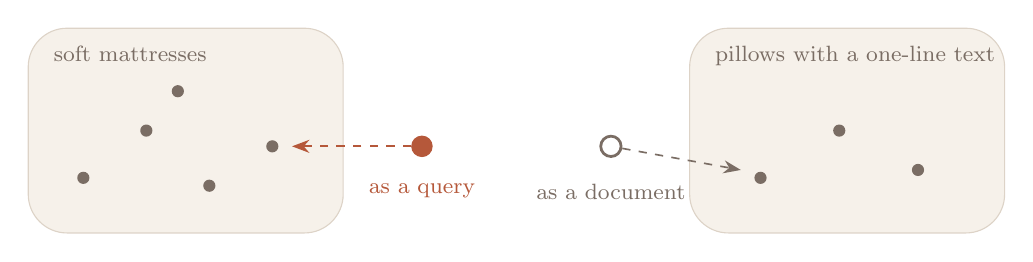
\begin{tikzpicture}[x=1cm, y=1cm]
  \draw[line, fill=paper, rounded corners=14pt]
    (0.0,0.0) rectangle (4.0,2.6);
  \node[lbl, anchor=north west] at (0.2,2.5) {soft mattresses};
  \draw[line, fill=paper, rounded corners=14pt]
    (8.4,0.0) rectangle (12.4,2.6);
  \node[lbl, anchor=north west] at (8.6,2.5)
    {pillows with a one-line text};
  \foreach \p in {(0.7,0.7),(1.5,1.3),(2.3,0.6),(3.1,1.1),(1.9,1.8)}
    \fill[muted] \p circle (2.2pt);
  \foreach \p in {(9.3,0.7),(10.3,1.3),(11.3,0.8)}
    \fill[muted] \p circle (2.2pt);
  \node[draw=accent, fill=accent, circle, inner sep=2.6pt]
    (q) at (5.0,1.1) {};
  \node[lbl, text=accent, anchor=north] at (5.0,0.75) {as a query};
  \node[draw=muted, fill=white, circle, inner sep=2.6pt, line width=1pt]
    (d) at (7.4,1.1) {};
  \node[lbl, anchor=north] at (7.4,0.75) {as a document};
  \draw[hotflow, dashed] (q) -- (3.35,1.1);
  \draw[flow, dashed] (d) -- (9.05,0.8);
\end{tikzpicture}
\caption{A sketch, not a measurement. The same sentence lands in a
different place depending on its task type. As a document it sits
near texts that look like it; as a query it sits near texts that
answer it.}
\label{fig:map}
\end{figure}

\subsection{Measured on all the test questions}

The same comparison was run on the 20 graded test questions, the
ones \code{check.py} reads from the file
\code{data/eval/product\_queries.json}. The full list is in
Appendix~\ref{app:all}; Table~\ref{tab:summary} has the averages.

\begin{table}[H]
\small
\begin{tabularx}{\textwidth}{@{}X c c c c@{}}
\toprule
 & \multicolumn{2}{c}{precision@5} & & \\
\cmidrule(lr){2-3}
Question embedded as & meaning (15) & language (5) & gap &
  top score \\
\midrule
\code{RETRIEVAL\_QUERY} & \textbf{0.99} & \textbf{0.96} &
  \textbf{+0.043} & 0.72 \\
\code{RETRIEVAL\_DOCUMENT} & 0.93 & 0.80 & +0.021 & 0.80 \\
\bottomrule
\end{tabularx}
\caption{Averages over the 20 graded questions, one run each. Both ways
find at least one right product in the top five for every question
(hit@5 is 1.00 for both). The \emph{gap} is the score of the best right
product minus the score of the best wrong one.}
\label{tab:summary}
\end{table}

Three things stand out.
\begin{enumerate}[leftmargin=1.4em, itemsep=3pt]
\item \textbf{The query type is better}, and most clearly on the Danish
  and German questions: 0.96 against 0.80. ``Matratze gegen
  Rückenschmerzen'' (German for ``mattress against back pain'') scores
  1.0 as a query and 0.6 as a document.
\item \textbf{The right answers stand out twice as clearly.} The
  \term{gap}{how far the best right product scores above the best wrong
  one. Bigger is safer.} doubles, from 0.021 to 0.043. A bigger gap
  means a small change in wording is less likely to push a wrong
  product to the top.
\item \textbf{Higher scores, worse results.} As a document, the top
  scores are higher (0.80 against 0.72) while the results are worse.
  Section~\ref{sec:score} explains why this is not a contradiction.
\end{enumerate}

\begin{keypoint}
Products are \emph{documents}; the customer's words are a
\emph{query}. Embed each with its own task type, and the question is
matched with what answers it, not with what looks like it.
\end{keypoint}

% ====================================================================
\section{Other task types}
\label{sec:types}

The store is \term{asymmetric}{the two sides of the comparison are
different kinds of text: a short need on one side, a description on the
other.}: a short need on one side, a product description on the other.
Not every application is like that.

Take a project management tool where every past project has a set of
cards: scope, stakeholders, schedule, budget, risks, communication
plan. A new project comes in with its own description, and the
question is ``which past projects were like this one?''. Now both sides
are the same kind of text: a project description against project
descriptions. The comparison is \term{symmetric}{both sides are the same
kind of text, and either could be swapped for the other.}, and nobody
is asking a question.

For that case the model has a separate task type, used on both sides.
Table~\ref{tab:types} lists the ones the Gemini embedding model offers.

\begin{table}[H]
\small
\begin{tabularx}{\textwidth}{@{}l X@{}}
\toprule
Task type & Use it when \\
\midrule
\code{RETRIEVAL\_QUERY} + \code{\_DOCUMENT} &
  a question looks for the text that answers it (this store) \\
\code{SEMANTIC\_SIMILARITY} &
  both sides are the same kind of text (similar past projects) \\
\code{CLASSIFICATION} &
  texts are sorted into fixed labels (``high risk'', ``low risk'') \\
\code{CLUSTERING} &
  texts are grouped with no labels given (families of projects) \\
\code{QUESTION\_ANSWERING} &
  a question is matched with passages that hold the answer \\
\code{FACT\_VERIFICATION} &
  a claim is matched with passages that support or refute it \\
\bottomrule
\end{tabularx}
\caption{Task types of \code{gemini-embedding-001}. The choice is a
starting point; a small test set decides.}
\label{tab:types}
\end{table}

One more lesson from the project example: embed each card on its own
and compare like with like, the new risk card with past risk cards and
the new scope with past scopes. One long text per project blurs
everything together, so a project with a similar budget but a
different scope would look half-similar to everything.

% ====================================================================
\section{What the score means}
\label{sec:score}

Each product card on the page shows a small number, for example
\emph{score 0.72}. What it means depends on which search produced it.

\subsection{Today: the keyword placeholder}

Until \code{search()} in \code{api/search.py} works, the API falls back
to a simple keyword search (\code{api/keyword\_search.py}) and the page
says ``keyword placeholder''. Its score is the share of the question's
words that appear in the product's text:
\[
  \text{score} \;=\;
  \frac{\text{question words found in the product}}
       {\text{all question words}}
\]

\begin{example}{Example}
The customer types \emph{grey wool rug}: three words.
\par\smallskip
\begin{tabularx}{\linewidth}{@{}X l r@{}}
A grey wool rug & grey, wool, rug: 3 of 3 & 1.00 \\
A blue wool rug & wool, rug: 2 of 3 & 0.67 \\
A grey sofa & grey: 1 of 3 & 0.33 \\
A grey couch & grey: 1 of 3 & 0.33 \\
\end{tabularx}
\par\smallskip
It counts words and knows nothing about meaning: a search for
\emph{couch} never finds a product called \emph{sofa}.
\end{example}

\subsection{After your search works: closeness in meaning}

Once \code{search()} works, the score is the \term{cosine
similarity}{how closely two vectors point the same way. With vectors of
length 1 it is just their dot product.} between the question's vector
and the product's vector: the number your matrix product
\code{index.vectors @ question} gives for that product. Higher means
closer in meaning. Three things about it are easy to get wrong.

\paragraph{It is not a percentage.} A score of 0.72 does not mean
``72\,\% relevant''. On this store, good matches land around 0.70 to
0.80 and poor ones a little lower. The range is narrow because all 500
texts are about furniture and already have much in common.

\paragraph{It only ranks.} A score is useful for one thing: deciding,
for \emph{one} question, whether product A is closer than product B.
A 0.72 for one question and a 0.72 for another cannot be compared.

\paragraph{No fixed cut-off.} Because of this, a rule such as ``only
show products above 0.75'' does not work. Table~\ref{tab:summary}
showed why: embedding the question as a document raised every score to
about 0.80 while making the results worse. The whole scale moved; the
order is what got worse. Figure~\ref{fig:line} shows this for the side
sleeper question.

\begin{figure}[H]
\centering
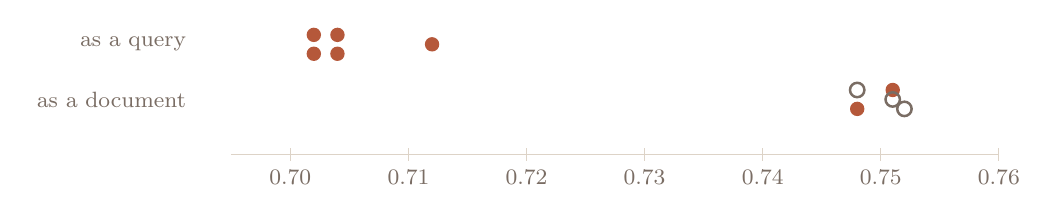
\begin{tikzpicture}[x=150cm, y=1cm]
  \def\lo{0.695}
  \draw[line, line width=0.6pt] (0,0) -- ({0.760-\lo},0);
  \foreach \v in {0.70, 0.71, 0.72, 0.73, 0.74, 0.75, 0.76}
    { \draw[line] ({\v-\lo},-0.08) -- ({\v-\lo},0.08);
      \node[lbl, below] at ({\v-\lo},-0.08) {\v}; }
  \node[lbl, anchor=east] at (-0.003,1.4) {as a query};
  \foreach \v/\dy in {0.712/0, 0.704/0.12, 0.704/-0.12, 0.702/0.12,
                      0.702/-0.12}
    \fill[accent] ({\v-\lo},{1.4+\dy}) circle (2.6pt);
  \node[lbl, anchor=east] at (-0.003,0.7) {as a document};
  \foreach \v/\dy in {0.751/0.12, 0.748/-0.12}
    \fill[accent] ({\v-\lo},{0.7+\dy}) circle (2.6pt);
  \foreach \v/\dy in {0.752/-0.12, 0.751/0, 0.748/0.12}
    \draw[muted, line width=0.9pt] ({\v-\lo},{0.7+\dy}) circle (2.6pt);
\end{tikzpicture}
\caption{Scores of the top five products for the side sleeper
question. Filled dots are right answers, rings are wrong ones. The
document row scores higher and still lets three pillows in.}
\label{fig:line}
\end{figure}

\begin{keypoint}
The score is a ranking signal for one question, not a measure of
quality. Compare scores within a question, never across questions or
settings.
\end{keypoint}

% ====================================================================
\section{Where filters come from}
\label{sec:filters}

A \term{filter}{a hard rule that removes products from the results, no
matter how close in meaning they are.} is a rule the results must obey,
such as ``only sofas'' or ``at most 5000~kr''. Your filter function in
\code{api/search.py} receives them as a \code{SearchFilters} with two
fields, \code{category} and \code{max\_price}, either of which can be
\code{None} for ``not set''. It does not care where they came from.
There are two places they can come from.

\subsection{From the page}

The customer clicks a category chip such as \emph{Sofa}, or picks a
maximum price. The page sends those choices to the API next to the
question, and the API turns them into
\code{SearchFilters(category="sofa", max\_price=5000)}. This is what
Step~1 does, and it is exact: a click means what it says.

\subsection{From the words}

A customer may instead type it all in one sentence:
\begin{quote}\itshape
A red comfortable sofa under 5000 dkk
\end{quote}
An embedding handles \emph{red}, \emph{comfortable} and \emph{sofa}
well, because those are meaning. It cannot handle \emph{under 5000
dkk}. To an embedding, that is a few words with a vague money feel; it
has no way to check that 4800 is below 5000, so a sofa at 9000~kr can
still come first. This is what the three \code{needs\_filter} test
questions show (``sofa under 4000 kr'', ``sofa that is not leather'',
``mattress 180x200''), and why \code{check.py} does not grade them.

The fix is to read the sentence \emph{before} searching, and split it
into the part that is meaning and the part that is a rule. That job
needs a different kind of model.

\subsection{Two kinds of model}

\begin{table}[H]
\small
\begin{tabularx}{\textwidth}{@{}l X X@{}}
\toprule
 & Embedding model & Text model \\
\midrule
Name & \code{gemini-embedding-001} & \code{gemini-3-flash-preview} \\
Call & \code{models.embed\_content} & \code{models.generate\_content} \\
Gives back & 768 numbers & text, or JSON in a shape you define \\
Reads ``5000'' as a number & no & yes \\
\bottomrule
\end{tabularx}
\caption{The embedding model turns text into a vector; only the text
model can read the sentence and fill in a form.}
\end{table}

\subsection{Structured output}

The text model can be made to answer in a fixed shape instead of
prose. This is called \term{structured output}{the model must reply
with data in a shape you define, not free text.}. It takes three parts.

\paragraph{1. Describe the answer as a class.} The same idea as
\code{Index}: a container with named slots.
\begin{lstlisting}[language=Python]
class SearchRequest(BaseModel):
    search_text: str                                 # the meaning part
    category: Literal["sofa", "mattress", ...] | None  # one of 8, or none
    max_price: float | None                          # a number, or none
\end{lstlisting}

\paragraph{2. Call the text model with the class as the schema.}
The class goes in as the \code{response\_schema}, next to an
instruction that says what to do:
\begin{lstlisting}[language=Python]
reply = client.models.generate_content(
    model="gemini-3-flash-preview",
    contents="A red comfortable sofa under 5000 dkk",
    config=types.GenerateContentConfig(
        system_instruction="Split the customer's search into "
            "search_text and filters. Only set a filter if the "
            "customer clearly says it.",
        response_mime_type="application/json",
        response_schema=SearchRequest))
\end{lstlisting}
The \code{response\_schema} forces the reply into that shape: valid
JSON, a category from the eight allowed, a price that is a number. The
model cannot answer ``Sure! It looks like you want a sofa\ldots''.

\paragraph{3. Use the parts.} The \code{search\_text} goes to
\code{embed\_query}; \code{category} and \code{max\_price} go into a
\code{SearchFilters} for your filter function. Figure~\ref{fig:flow}
shows the whole path.

\begin{figure}[H]
\centering
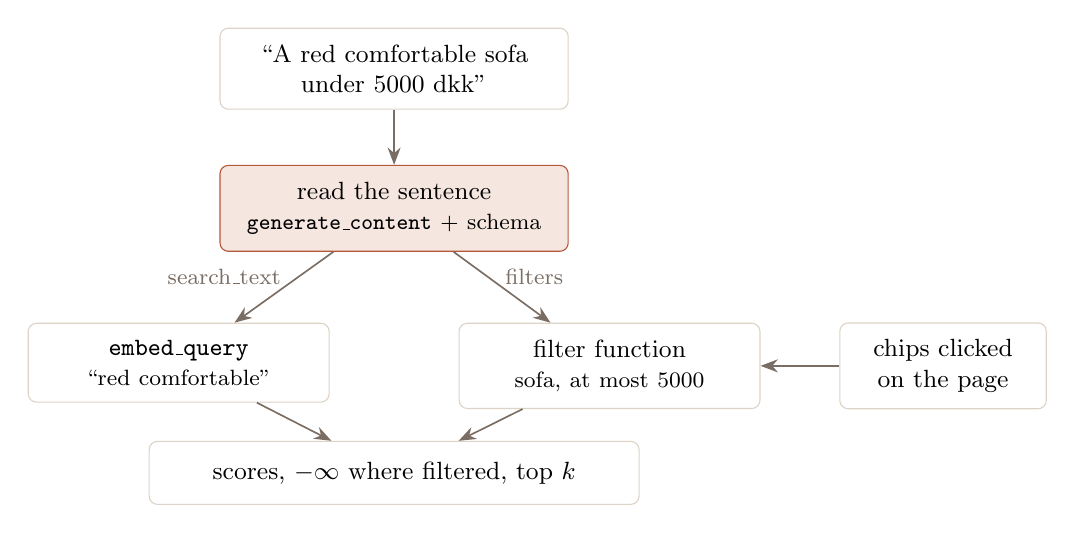
\begin{tikzpicture}[node distance=7mm and 9mm]
  \node[box, text width=40mm] (q)
    {``A red comfortable sofa\\ under 5000 dkk''};
  \node[hot, below=of q, text width=40mm] (x)
    {read the sentence\\ \footnotesize\code{generate\_content} + schema};
  \node[box, below left=9mm and -14mm of x, text width=34mm] (e)
    {\code{embed\_query}\\ \footnotesize``red comfortable''};
  \node[box, below right=9mm and -14mm of x, text width=34mm] (f)
    {filter function\\ \footnotesize sofa, at most 5000};
  \node[box, below=24mm of x, text width=58mm] (s)
    {scores, $-\infty$ where filtered, top $k$};
  \node[box, right=10mm of f, text width=22mm] (c)
    {chips clicked\\ on the page};
  \draw[flow] (q) -- (x);
  \draw[flow] (x) -- node[lbl, left, pos=0.35] {search\_text\ } (e);
  \draw[flow] (x) -- node[lbl, right, pos=0.35] {\ filters} (f);
  \draw[flow] (c) -- (f);
  \draw[flow] (e) -- (s);
  \draw[flow] (f) -- (s);
\end{tikzpicture}
\caption{The highlighted step is new; the rest is Step~1 as you are
writing it. Filters can arrive from the words, from the page, or both.}
\label{fig:flow}
\end{figure}

When the customer both clicks a filter and types one, the two are
merged. A sensible rule is that the click wins, because it is the more
deliberate of the two.

\subsection{It needs testing too}

The model reads well but not perfectly. Four searches, run once:

\begin{table}[H]
\small
\begin{tabularx}{\textwidth}{@{}X l l X@{}}
\toprule
Search & Category & Max price & Comment \\
\midrule
A red comfortable sofa under 5000 dkk & sofa & 5000 &
  right; text became ``red comfortable'' \\
billig madras under 2000 kr & mattress & 2000 &
  right; but ``under 2000 kr'' stayed in the text \\
something cosy for the living room floor & rug & none &
  \textcolor{accent}{a guess: rug was never said} \\
pillow for neck pain & pillow & none & right \\
\bottomrule
\end{tabularx}
\caption{Filters read from the words by \code{gemini-3-flash-preview}.
``Billig madras'' is Danish for ``cheap mattress''.}
\label{tab:extract}
\end{table}

The third row matters most. The instruction said ``only if the
customer clearly says it'', and the model guessed anyway. A filter is a
hard cut, so a wrong filter hides every other product, however good.
A wrong filter is worse than no filter. That is why this step gets its
own test questions with known right answers, measured the same way as
the search: the plan for Step~3.

\begin{keypoint}
Filters from the page are exact; filters from the words are read by a
text model with structured output, before the search. Your filter
function stays the same either way: it only ever sees a
\code{SearchFilters}.
\end{keypoint}

% ====================================================================
\clearpage
\appendix
\section{All 20 graded questions}
\label{app:all}

\begin{table}[H]
\footnotesize
\begin{tabularx}{\textwidth}{@{}X l c r c r@{}}
\toprule
 & & \multicolumn{2}{c}{as a query} & \multicolumn{2}{c}{as a document} \\
\cmidrule(lr){3-4}\cmidrule(l){5-6}
Question & Kind & p@5 & top & p@5 & top \\
\midrule
a mattress that helps with back pain & meaning & 1.0 & 0.737 & 1.0 & 0.801 \\
madras der hjælper mod ondt i ryggen & language & 1.0 & 0.788 & \textcolor{accent}{0.8} & 0.832 \\
Matratze gegen Rückenschmerzen & language & 1.0 & 0.728 & \textcolor{accent}{0.6} & 0.806 \\
something soft to sleep on if I sleep on my side & meaning & 1.0 & 0.712 & \textcolor{accent}{0.4} & 0.752 \\
mattress that does not get hot at night & meaning & 1.0 & 0.698 & 1.0 & 0.778 \\
pillow for neck pain & meaning & 1.0 & 0.708 & 1.0 & 0.785 \\
bedding for someone allergic to dust mites & meaning & 1.0 & 0.681 & 1.0 & 0.763 \\
varm dyne til vinteren & language & 1.0 & 0.772 & \textcolor{accent}{0.8} & 0.840 \\
duvet for hot summer nights & meaning & 1.0 & 0.725 & \textcolor{accent}{0.8} & 0.799 \\
a couch my guests can sleep on & meaning & 1.0 & 0.716 & 1.0 & 0.778 \\
Schlafsofa für Gäste & language & 1.0 & 0.720 & 1.0 & 0.800 \\
sofa that survives a dog and two kids & meaning & 1.0 & 0.690 & 1.0 & 0.793 \\
sofa where I can put my legs up & meaning & 1.0 & 0.717 & 1.0 & 0.798 \\
big table for family dinners that can get longer & meaning & 1.0 & 0.728 & 1.0 & 0.814 \\
spisebord i massiv eg & language & 0.8 & 0.771 & 0.8 & 0.892 \\
chair for working from home without back ache & meaning & 1.0 & 0.702 & 1.0 & 0.812 \\
outdoor furniture that can stay out in the rain & meaning & 1.0 & 0.699 & 1.0 & 0.813 \\
rug I can put in the washing machine & meaning & 0.8 & 0.704 & 0.8 & 0.788 \\
rug for my balcony & meaning & 1.0 & 0.734 & 1.0 & 0.815 \\
wool rug & meaning & 1.0 & 0.704 & 1.0 & 0.809 \\
\midrule
\textbf{Average} & & \textbf{0.98} & 0.722 & 0.90 & 0.803 \\
\bottomrule
\end{tabularx}
\caption{Precision@5 and the highest score for each question, with the
question embedded each way. Where the document type does worse, the
number is marked. One run; the product vectors are the same in both
columns.}
\end{table}

\end{document}
